\documentclass[12pt, titlepage]{article}
\usepackage[a4paper,margin=.75in]{geometry}
\usepackage{tgtermes}
\usepackage{amsmath}
\usepackage{setspace}
\usepackage{placeins}
\usepackage{listings}
\usepackage{color}
\usepackage{fancyhdr}
\usepackage{graphicx}
\usepackage[parfill]{parskip}
\usepackage{hyperref}
\hypersetup{
    colorlinks=true,
    linkcolor=blue,
    filecolor=magenta,      
    urlcolor=cyan,
}

\definecolor{dkgreen}{rgb}{0,0.6,0}
\definecolor{gray}{rgb}{0.5,0.5,0.5}
\definecolor{mauve}{rgb}{0.58,0,0.82}

\lstset{frame=none,
  language=Java,
  aboveskip=3mm,
  belowskip=3mm,
  showstringspaces=false,
  columns=flexible,
  basicstyle={\small\ttfamily},
  numbers=none,
  numberstyle=\tiny\color{gray},
  keywordstyle=\color{blue},
  commentstyle=\color{dkgreen},
  stringstyle=\color{mauve},
  breaklines=true,
  breakatwhitespace=true,
  tabsize=3
}

\pagestyle{fancyplain}
\lhead{Sean Connor}
\chead{Project 3 - Analysis}
\rhead{30 July 2018}

\title{Project 3 Analysis}
\author{Sean Connor \\ \\ 605.202 Data Structures \\ \\ 30 July 2018}
\date{}
\singlespacing

\begin{document}

\maketitle




\section {Data Structures}

The requirements defined for this project include the following:
\begin{itemize}
	\item Read a matrix, print it out, compute and print the determinant
	\item Evaluate multiple matrices on a single execution
	\item Handle matrices up to and including those of order 6
	\item Mandatory use of linked list type structure to store the matrix
\end{itemize}

A significant portion of this project includes code that was created previously for Project 2 (determinant of matrix using recursive method), such as methods to read the input file and create the output file. However, due to freedom to use iterative or recursive methods, my chosen method of determinant calculation is different.
 
The required data structure for this project was a linked list type structure. I implemented the linked list using two Java classes - Node and LinkedList. 

Node was implemented as a Java generic; that is, it is of the form Node$<$T$>$. A Node object contains a variable of type T to store the data, a ``pointer" to the previous Node, and a ``pointer" to the next Node. This makes the linked list utilizing the Node object a doubly-linked list, as each node contains a forward pointer and a backward pointer.
 
LinkedList was also implemented as a Java generic. The purpose for this is to allow the LinkedList class to have the capability to handle objects of any type (i.e. Integer, Double, String, etc). I elected not to implement the LinkedList with a header node, as it was not a requirement for this project and did not provide any significant benefit. However, the LinkedList class does contain ``pointers" to the first and last Nodes. 

There were a number of implementation methods considered for storing a matrix in a LinkedList. Some possibilities include:
\begin{itemize}
	\item List of Lists - The main LinkedList stores LinkedLists in each Node's data section, where each secondary LinkedList represents a row in the matrix.
	\item Array of LinkedLists - The same premise as above, where each index of the array stores a LinkedList that represents a row in the matrix.
	\item A single LinkedList - The values of the matrix are read row by row, left to right for each row, and stored as Nodes in one long LinkedList.
\end{itemize}

I chose to store the matrix as a single LinkedList$<$Double$>$ for simplicity. To illustrate this, see the following figure.

\[
\begin{bmatrix}
    1 & 0 & 0 \\
    0 & 2 & 0  \\
    0 & 0 & 3 
\end{bmatrix}
\Longleftrightarrow
\begin{bmatrix}
    1 & 0 & 0 & 0 & 2 & 0 & 0 & 0 & 3
\end{bmatrix}
\]

The LinkedList class contains a variety of methods - some that are necessary for functionality as a LinkedList and some that are helpful in dealing with matrices. Some important methods are:
\begin{itemize}
	\item insert(T data) - inserts a Node with data of type T at the end of the LinkedList.
	\item matrixToListIndex(int row, int col) - returns the index of the LinkedList corresponding to the given row and column (i.e. for a matrix of order 3, matrixToListIndex(0,0) would return 0 and matrixToListIndex(1,1) would return 4).
	\item setValue(int row, int col, T data) - sets the data value of Node corresponding to given matrix element to `data'. 
	\item getValue(int row, int col) - returns the data value of Node corresponding to given matrix element.
\end{itemize}




\section{General Strategy}

The recursive algorithm used in Project 2 is described in one of the project description files (ALT3.2.6.pdf). It is restated here for convenience.

\begin{equation*}
\textrm{det}(a) = \sum_j \textrm{power}(-1, i+j) \times a[i,j] \times \textrm{det}(\textrm{minor}(a[i,j])), \textrm{for any i}
\end{equation*}

This algorithm is not very efficient, becoming impractical for matrices beyond about order 12-15. I elected to use a different method for determinant calculation. The main reasons for this were (a) because I was not satisfied with the performance of the recursive algorithm used previously, and (b) because I wanted to practice implementing a different method. Research from the previous project revealed that Gaussian Elimination is a relatively simple and efficient method for determinant calculation, and so this is what I implemented for this project. I chose to implement this as an iterative method, primarily because I am more comfortable with iterative methods and it was simplest to implement.

The general strategy of Gaussian Elimination is to reduce a matrix to an upper triangular matrix using elementary row operations. This is perhaps best demonstrated with an example.

\[
\begin{bmatrix}
    1 & 2 & 3 \\
    4 & 5 & 6  \\
    7 & 8 & 9 
\end{bmatrix}
\longrightarrow
\begin{array}[]{r}
     [4, 5, 6]  \\
- \ 4[1, 2, 3] \\ \hline
    [0, -3, -6]
\end{array}
\&
\begin{array}[]{r}
     [7, 8, 9]  \\
- \ 7[1, 2, 3] \\ \hline
    [0, -6, -12]
\end{array}
\longrightarrow
\begin{bmatrix}
    1 & 2 & 3 \\
    0 & -3 & -6  \\
    0 & -6 & -12 
\end{bmatrix}
\]

\[
\begin{bmatrix}
    1 & 2 & 3 \\
    0 & -3 & -6  \\
    0 & -6 & -12 
\end{bmatrix}
\longrightarrow
\begin{array}[]{r}
     [0, -6, -12]  \\
- \ 2[0, -3, -6] \\ \hline
    [0, 0, 0]
\end{array}
\longrightarrow
\begin{bmatrix}
    1 & 2 & 3 \\
    0 & -3 & -6  \\
    0 & 0 & 0 
\end{bmatrix}
\]

\[
\text{det} = \prod_{i=1}^{size} A_{ii} = 1 \times -3 \times 0 = 0
\]

The input was read line by line from a text file using a combination of BufferedReader, InputSteamReader, and FileInputStream. The input text file must be formatted correctly, otherwise the program will produce an error message. Typical errors include empty lines in the text file, improper specification of size, and matrices that are not square. The first line of the input file is read normally. This line specifies the size of the first matrix. After this, the program reads n lines, where n is equal to specified matrix size. After reading each line, the String.split() and Integer.parseInt() methods are employed to split the String into a String[] of numbers, which are then converted to int and placed in an int[][] matrix. Finally, as the reader moves through the input file and calculated the determinants, the matrix information (including determinant) is printed to the console and appended to a StringBuilder object, which is returned and written to specified output file in the main() method using BufferedWriter/OutputStreamWriter/FileOutputStream.





\section{Algorithm Efficiency}

From the previous project, we saw that the recursive algorithm performed with an efficiency of about O(N!), and it rapidly became unusable as matrix size increased beyond 12-15. With the Gaussian Elimination algorithm, determinant calculation were performed orders of magnitude faster. While extensive testing was not performed, for a single matrix of order 25, the determinant was calculated between 0.06 and 0.09 seconds. For the required order 6 test case, the Gaussian Elimination algorithm with LinkedList was on average twice as fast as the recursive algorithm with array. For the ``factorial matrix" (see below for example) of order 11, the Gaussian Elimination algorithm was on average about 36000 times faster than the recursive algorithm. This difference increases exponentially as matrix order increases.

\[
\begin{bmatrix}
	1 & 0 & 0 & 0 & 0 \\
	0 & 2 & 0 & 0 & 0 \\
	0 & 0 & 3 & 0 & 0 \\
	0 & 0 & 0 & 4 & 0 \\
	0 & 0 & 0 & 0 & 5 
\end{bmatrix}
\]

Here is a comparison of the average time to completion (three runs averaged) for the Gaussian implementation used in this project versus the Recursive implementation as used in Project 2. I can't account for the strange ``bumps" seen in the Gaussian curve; however, it is clear that the Gaussian method is substantially faster. As far as space complexity goes, I suspect that the Gaussian method is better than the recursive method, as the Gaussian method simply changes values of the LinkedList Nodes, rather than create new arrays/LinkedLists for submatrices as used in the recursive method.

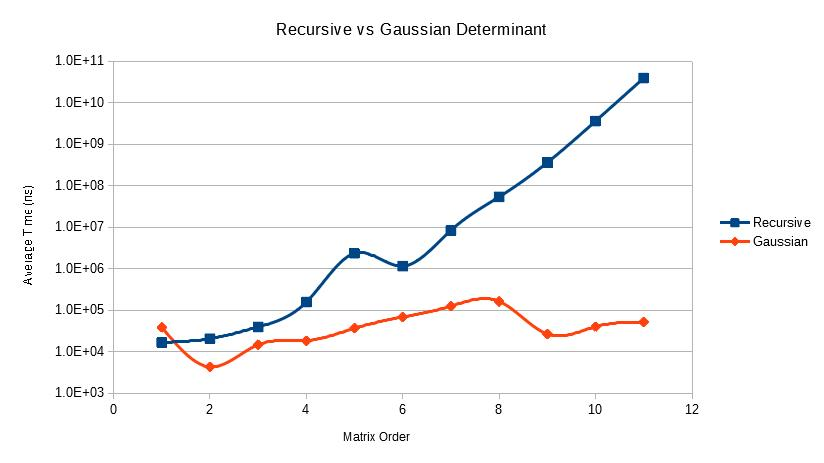
\includegraphics[width=\textwidth]{compare}




\section{Lessons Learned}

List of Lists or Array of Lists may be faster due to sequential access of LinkedList. This is particularly true for larger matrices. For example if there was a matrix of order 1000, then to access matrix(1000,999) if stored in a single singly-linked LinkedList, one would need to move sequentially to the 1000\textsuperscript{2} - 1 = 999999\textsuperscript{th} element, for a total of 999999 operations. Alternatively, if implemented as a List of Lists, then one would move sequentially through the primary LinkedList to the final row, and then move sequentially through the secondary LinkedList to the 999\textsuperscript{th} element, for a total of 1999 operations. However, for this project such optimization/performance was not necessary, and implementing as a single LinkedList to store the entire matrix provided a very simple solution.
 
The most significant performance gains were seen in changing the determinant calculation algorithm from the recursive one provided in project document ALT3.2.6.pdf to the Gaussian Elimination with partial pivoting algorithm. As mentioned, I elected to implement the Gaussian Elimination method as an iterative method. From what I understand, any recursive method can be made into an iterative method and vice versa. However, in popular programming languages like Java, C, and Python, iterative methods are generally more efficient than recursive methods [1]. Aside from this, I am simply more familiar/comfortable using iteration.
 
This project provided a good lesson in implementing a linked list data structure, and in seeing how it could be easily used to store data such as a matrix. While I still like the simplicity of arrays/ArrayList, LinkedList definitely has some advantages. As with many things, it seems to depend upon intended use, with LinkedList being better for insertion/removal of elements and ArrayList being better for accessing elements.  

\newpage

\section{References}
\begin{enumerate}
	\item ``Is recursion ever faster than looping?" StackOverflow. \url{https://stackoverflow.com/questions/2651112/is-recursion-ever-faster-than-looping}
\end{enumerate}

\end{document}